\documentclass[a4paper,12pt]{article}  
\usepackage[utf8]{inputenc}            
\usepackage[T1]{fontenc}              
\usepackage{lmodern}                  
\usepackage{xcolor}                   
\usepackage{graphicx}                 
\usepackage{hyperref}                 
\usepackage{amsmath}                  
\usepackage{geometry}                 
\usepackage{titling}                  
\usepackage{float}                    
\usepackage{titlesec}                 
\usepackage{xurl}
\usepackage{subcaption} 

\usepackage{fancyhdr}                 
\usepackage[portuguese]{babel}     
\usepackage{tikz}
\usepackage{booktabs}
\usepackage{tabularx}
\usepackage{longtable}
\usepackage{xltabular}
\usetikzlibrary{shapes, arrows, positioning, calc}

% Configuração da geometria da página  
\geometry{top=2cm, bottom=2cm, left=3cm, right=3cm}  

% Configuração do hyperref  
\hypersetup{  
    colorlinks=true,  
    linkcolor=blue,  
    urlcolor=blue  
}  

% Configuração do cabeçalho e rodapé  
\pagestyle{fancy}  
\fancyhf{}  
\fancyhead[L]{Universidade Tecnológica Federal do Paraná}  
\fancyhead[R]{Oficina de Integração 2}  
\fancyfoot[C]{\thepage}  
\renewcommand{\headrulewidth}{0.4pt}  
\renewcommand{\footrulewidth}{0.4pt}  

% Customização dos títulos das seções  
\titleformat{\section}  
  {\normalfont\Large\bfseries\color{black}}{\thesection}{1em}{}  
\titleformat{\subsection}  
  {\normalfont\large\bfseries\color{black}}{\thesubsection}{1em}{}  

\date{\today}  

\begin{document}  

\vspace{1em}  
\begin{center}  
    \Large\textbf{Projeto Jennie: Servidor NAS de Baixo Consumo e  Alta Confiabilidade} \\
\end{center} 
\vspace{1em}  

% Autores e contatos  
\begin{center}  
    \textbf{Fernando Frare Vieira} \\  
    \href{mailto:fernandofrarevieira@alunos.utfpr.edu.br}{fernandofrarevieira@alunos.utfpr.edu.br} \\  
    +55 41 99900-6940 \\[1.5em]  
    \textbf{Gabriel Affonso Borges Caballero} \\  
    \href{mailto:gabrielaffonso@alunos.utfpr.edu.br}{gabrielaffonso@alunos.utfpr.edu.br} \\  
    +55 41 99151-3335\\[1.5em]  
    \textbf{Marco Vieira Busetti} \\  
    \href{mailto:marcovieirabusetti@alunos.utfpr.edu.br}{marcovieirabusetti@alunos.utfpr.edu.br} \\  
    +55 41 99798-4695  
\end{center}  

\vspace{1em}
\begin{center}  
    \today  \\[1cm]
    \href{https://www.notion.so/JENNIE-NAS-Open-Source-330dca6860fa807d94e1dabd933a0dda}{Website do Projeto}
\end{center}
\vspace{2em}

% --- SEÇÃO: INTRODUÇÃO ---  
\section{Introdução}  
Atualmente, os serviços convencionais de armazenamento em nuvem (\textit{cloud storage}) apresentam desafios significativos no que diz respeito à privacidade dos dados, limitação de controle por parte do usuário e ineficiência energética \cite{zissis2012}. Para mitigar esses problemas, o mercado oferece soluções de \textit{Network Attached Storage} --- NAS voltadas para o consumidor final, permitindo a hospedagem de dados na própria residência. 

Contudo, essas soluções comerciais frequentemente se baseiam em hardware e software proprietários, o que caracteriza um modelo de "caixa preta" (\textit{vendor lock-in}) \cite{shapiro1999}. Além de restringir a verdadeira privacidade e o controle absoluto do sistema, os produtos de NAS tradicionais possuem um custo de aquisição elevado e um consumo de energia considerável para operações contínuas \cite{berl2010}.

Diante desse cenário de problemas em cascata, este projeto propõe o desenvolvimento de um servidor NAS eficiente, transparente e acessível, fundamentado em uma placa Raspberry Pi 5 \cite{upton2014}. A arquitetura funcionará sob um sistema operacional customizado de código livre e aberto, garantindo total transparência e otimização de recursos. Adicionalmente, o projeto engloba a construção de módulos eletrônicos dedicados, incluindo um no-break (\textit{Uninterruptible Power Supply} --- UPS) e controle de refrigeração ativa, assegurando a estabilidade e a integridade do hardware.


\begin{figure}[htbp]
    \centering
    \begin{subfigure}[b]{0.48\textwidth}
        \centering
        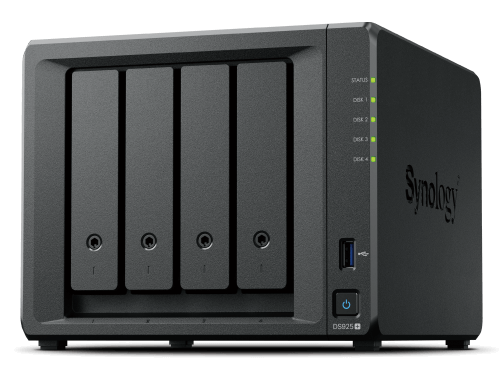
\includegraphics[width=\textwidth]{images/synology.png}
        \caption{NAS Comercial (Exemplo Synology).\\ \vspace{0.1cm} \scriptsize Fonte: Site da Synology (\url{https://www.synology.com}).}
        \label{fig:synology}
    \end{subfigure}
    \hfill
    \begin{subfigure}[b]{0.48\textwidth}
        \centering
        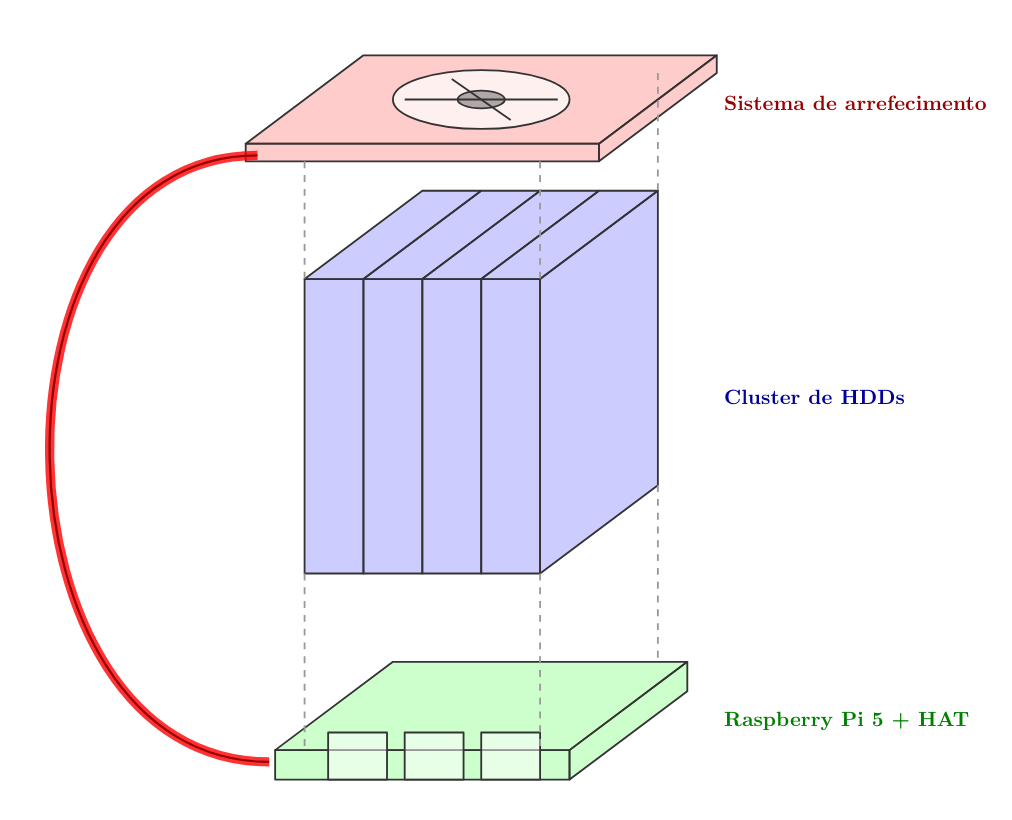
\includegraphics[width=\textwidth]{images/esquema_nas.png}
        \caption{Esquemático da montagem do Projeto Jennie.}
        \label{fig:esquema_nas}
    \end{subfigure}
    
    \caption{Comparação entre um sistema comercial e a montagem customizada proposta.}
    \label{fig:comparacao_nas}
\end{figure}


 %--- SEÇÃO: DESCRIÇÃO GERAL ---  
\section{Descrição Geral}  
O projeto consiste em um sistema de armazenamento estruturado em três componentes principais: hardware de processamento (Raspberry Pi 5), módulos eletrônicos de suporte e um ecossistema de software customizado. A Raspberry Pi atua como o núcleo do sistema, interligando o arranjo de discos rígidos através de barramentos de alta velocidade (\textit{Peripheral Component Interconnect Express} --- PCIe). Para viabilizar a operação 24/7 (funcionamento ininterrupto) de maneira confiável, um circuito no-break incorpora o gerenciamento de baterias e circuitos lógicos para acionamento das ventoinhas conforme a demanda térmica do processador e dos discos. \\
Do ponto de vista funcional, o sistema provê ao usuário uma plataforma centralizada para:
\begin{itemize}
\item \textbf{Gestão de Dados e Soberania Digital:} Armazenamento, organização e exploração de arquivos via rede local ou remota, utilizando protocolos seguros e interface web dedicada.
\item \textbf{Orquestração de Microserviços:} Capacidade de hospedar e gerenciar aplicações isoladas (contêineres — ambientes de execução isolados por software), como automações residenciais, bots de monitoramento e websites.
\item \textbf{Resiliência Operacional:} Garantia de disponibilidade através de um sistema de UPS (no-break) integrado, que monitora a rede elétrica e assegura o funcionamento contínuo ou o desligamento seguro em caso de falhas.
\end{itemize}

% --- SEÇÃO: DIAGRAMA DE BLOCOS ---  
\begin{figure}[H]  
    \centering  
    % Adicione o diagrama de blocos real na pasta images
    \makebox[\textwidth][c]{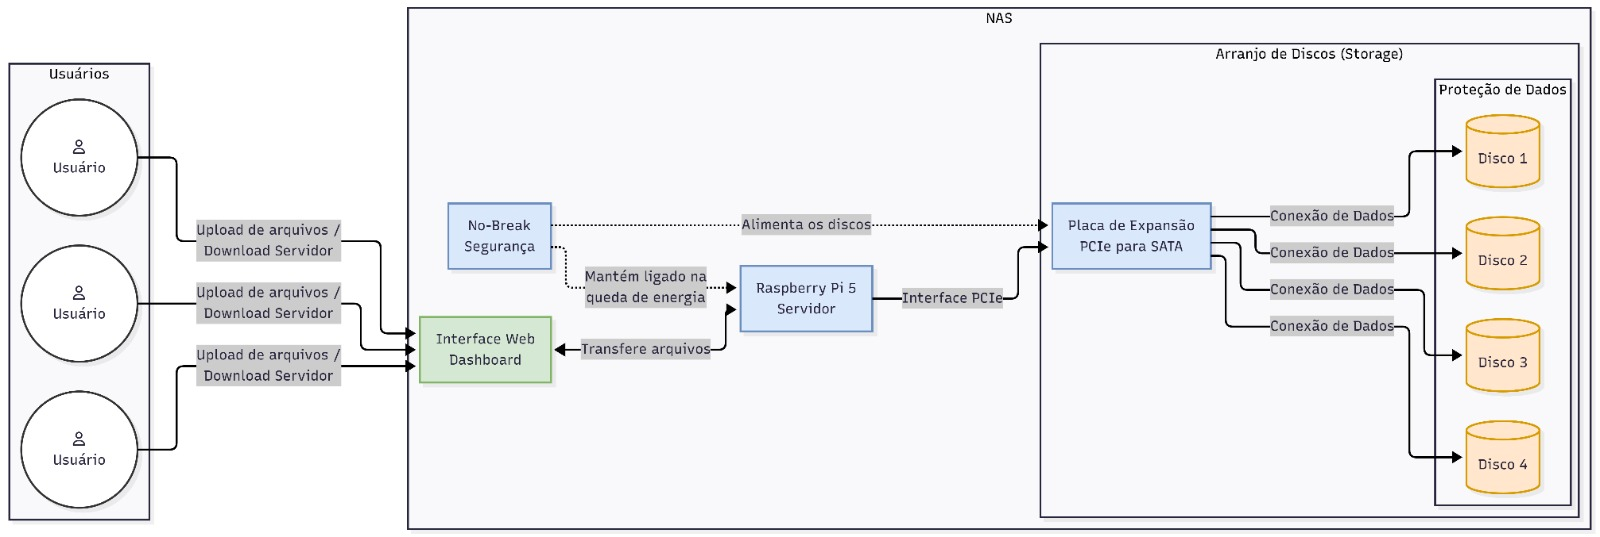
\includegraphics[width=1.2\textwidth]{images/diagrama.jpg}}
    \caption{Diagrama de Blocos da Arquitetura do NAS}  
    \label{fig:diagrama}  
\end{figure}  

% --- SEÇÃO: REQUISITOS ---
\section{Requisitos Funcionais e Não-Funcionais}

\subsection{Requisitos Funcionais (RF)}
\begin{itemize}
    \item \textbf{RF01 - Gerenciamento de Armazenamento:} O sistema deve ser capaz de reconhecer, formatar e gerenciar um arranjo de até 4 discos rígidos (\textit{Hard Disk Drives} --- HDDs) de 2.5". A escolha exclusiva por HDDs justifica-se pelo foco do projeto em alta densidade de armazenamento e soberania de dados com baixo custo de aquisição \cite{berl2010}. Visto que o gargalo de desempenho para o uso doméstico reside na interface de rede e no barramento PCIe-to-SATA (\textit{Serial ATA}) compartilhado \cite{halfacree2023}, o uso de SSDs (\textit{Solid State Drives} --- unidades de armazenamento em estado sólido) elevaria o custo total sem proporcionar ganho perceptível em aplicações de \textit{cold storage} (dados raramente acessados, priorizando baixo custo por GB) e servidores de mídia.
    \item \textbf{RF02 - Compartilhamento de Rede:} O sistema deve prover o acesso aos arquivos através da rede local (ou externa), permitindo leitura e escrita por diferentes dispositivos de forma segura.
    \item \textbf{RF03 - Controle de Acesso e Usuários:} O sistema deve permitir a criação de múltiplos usuários, gerenciando diferentes níveis de permissão de acesso a diretórios específicos.
    \item \textbf{RF04 - Segurança Física do Sistema:} O NAS deve incorporar mecanismos eletrônicos (no-break e controle térmico) que garantam a consistência da operação contra quedas de energia e sobreaquecimento.
    \item \textbf{RF05 - Hospedagem:} O sistema deve permitir a execução de serviços em ambientes isolados (contêineres), garantindo que falhas em uma aplicação não afetem o sistema operacional \textit{host} (sistema hospedeiro).
    \item \textbf{RF06 - Monitoramento e Dashboard:} O sistema deve disponibilizar uma interface web para visualização em tempo real das métricas de saúde (temperatura, tensão) e performance (uso de CPU (\textit{Central Processing Unit}), RAM (\textit{Random Access Memory}) e discos), além de permitir a configuração de alertas proativos em casos de anomalia.
    \item \textbf{RF08 - Gerenciamento de Serviços:} A interface web deve permitir ao usuário iniciar, parar e visualizar o status dos contêineres de microserviços.
    \item
    \textbf{RF07 - Recuperação:} O sistema deve possuir uma rotina automática de verificação e reparo do sistema de arquivos após quedas de energia inesperadas \cite{prabhakaran2005}.
\end{itemize}

\subsection{Requisitos Não-Funcionais (RNF)}
\begin{itemize}
    \item \textbf{RNF01 - Desempenho e Eficiência:} O sistema operacional deve ser enxuto e otimizado para a arquitetura \textit{Advanced RISC Machine} (ARM) embarcada, com baixo consumo de recursos e priorização da alocação de memória para aplicações do usuário.
    \item \textbf{RNF02 - Privacidade e Segurança Lógica:} A comunicação externa e a autenticação devem utilizar protocolos criptografados (ex: \textit{Transport Layer Security/Secure Sockets Layer} (TLS/SSL), \textit{Secure Shell} (SSH) \cite{rfc4251}), garantindo que os dados em trânsito e as aplicações de servidor não sejam interceptados.
    \item \textbf{RNF03 - Confiabilidade de Dados:} O gerenciamento de armazenamento deve utilizar um sistema de arquivos moderno (ex: Btrfs (com \textit{checksums} (somas de verificação de integridade) e detecção de \textit{bit rot}) ou ext4 (sistema padrão do Linux, sem \textit{checksums} nativos) com redundância) com suporte à verificação de integridade e prevenção contra corrupção silenciosa de dados (\textit{bit rot} — corrupção silenciosa de dados sem sinalização ao usuário) \cite{rodeh2013}.
    \item \textbf{RNF04 - Autonomia e Tolerância a Falhas:} O módulo de energia (no-break) deve manter o NAS operacional por 5 minutos após uma interrupção da rede elétrica, tempo suficiente para a conclusão do processo de \textit{shutdown} seguro, prevenindo perda de blocos em disco.
    \item \textbf{RNF05 - Estrutura e Concepção Mecânica:} O sistema deverá dispor de uma estrutura mecânica para conter o Raspberry Pi 5 e seus demais módulos, tais como refrigeração, circuito no-break, entre outros.
    \item
    \textbf{RNF06 - Escalabilidade Térmica:} O sistema de arrefecimento deve ser capaz de manter a temperatura abaixo do limite de \textit{thermal throttling} (redução de frequência do processador para prevenir danos por calor) mesmo sob carga de 100\% de CPU e I/O de disco por 30 minutos.
    \item \textbf{RNF07 - Arquitetura de Micro-Backend} A camada de gerenciamento deve utilizar um micro-backend de baixo \textit{overhead} (custo computacional adicional além da tarefa principal) (ex: Go ou Python), garantindo tempos de resposta inferiores a 200ms para requisições de status do sistema.
\end{itemize}

\subsection{Anti-Requisitos (AR)}
Os itens a seguir delimitam explicitamente o que \textbf{não faz parte} do escopo deste projeto, evitando expectativas incompatíveis com as limitações do hardware escolhido e com os objetivos da disciplina.
\begin{itemize}
    \item \textbf{AR01 - Sincronização com Nuvem:} O sistema não incluirá integração nativa com serviços de armazenamento em nuvem (ex: Google Drive, Dropbox, OneDrive). O foco do projeto é a soberania local dos dados; integrações externas podem ser adicionadas pelo usuário via contêineres, mas não serão desenvolvidas nem suportadas pela equipe.
    \item \textbf{AR02 - Criptografia Total de Disco:} O sistema não implementará criptografia completa de disco (\textit{full-disk encryption}). A sobrecarga de criptografia/descriptografia por software na arquitetura ARM reduziria significativamente o \textit{throughput} de leitura e escrita, inviabilizando o uso como servidor de arquivos.
    \item \textbf{AR03 - Expansão Além de 4 Discos:} O sistema não suportará mais de 4 discos rígidos de 2.5". A limitação é imposta pelo barramento PCIe da Raspberry Pi 5 e pela controladora SATA utilizada; expandir além disso exigiria hardware adicional fora do escopo.
    \item \textbf{AR04 - Interface Gráfica Local (Desktop):} O sistema operacional não contará com ambiente gráfico (desktop) instalado no próprio NAS. Toda a interação com o usuário será feita via interface web ou SSH remoto, mantendo o consumo de recursos do SO no mínimo.
\end{itemize}


% --- SEÇÃO: INTEGRAÇÃO ---
\section{Integração de Disciplinas}  
O desenvolvimento deste sistema exige uma abordagem multidisciplinar, conectando diversas disciplinas encontradas no curso de Engenharia de Computação da UTFPR:
\begin{itemize}
    \item \textbf{Sistemas Operacionais:} Construção e compilação de uma distribuição Linux customizada, configuração e compilação do \textit{kernel} (núcleo do sistema operacional) e gerenciamento de processos e sistemas de arquivos \cite{tanenbaum2015}.
    \item \textbf{Redes de Computadores:} Configuração de protocolos de compartilhamento, roteamento interno e exposição segura de serviços para redes externas.
    \item \textbf{Sistemas Embarcados \& Eletrônica Geral 1:} Interfaceamento da Raspberry Pi com o hardware customizado, condicionamento de sinais e dimensionamento de fontes chaveadas (conversores de tensão de alta eficiência) e circuitos de carga/descarga de baterias para o no-break.
    \item \textbf{Circuitos Digitais:} Controle PWM (\textit{Pulse Width Modulation} --- Modulação por Largura de Pulso) para refrigeração e lógica digital para os sensores do hardware de suporte.
    \item \textbf{Banco de Dados:} Estruturação dos dados utilizados pelos serviços hospedados no NAS e gerenciamento das permissões de acesso e metadados.
    \item \textbf{Engenharia de Software:} Aplicação de metodologias ágeis no ciclo de vida do desenvolvimento, levantamento de requisitos e versionamento do código \cite{sommerville2011}.
\end{itemize}

\vspace{1em}  

% --- SEÇÃO: DESCRIÇÃO DO SOFTWARE ---  
\section{Descrição do Sistema}
\subsection{Descrição do Software}
O ecossistema de software deste projeto é dividido em quatro camadas:  
\begin{itemize}  
    \item \textbf{Sistema Operacional:} Utilização da distribuição Gentoo Linux (distribuição compilada a partir do código-fonte, resultando em um sistema enxuto e otimizado para o hardware) como base, mas customizada para ser desprovida de pacotes não essenciais, com \textit{kernel} focado em inicialização rápida e baixo \textit{overhead}.
    \item \textbf{I/O (\textit{Input/Output} --- Entrada/Saída) e Rede:} \textit{Daemons} (processos em segundo plano que gerenciam serviços contínuos) responsáveis por expor o armazenamento, como o servidores diversos e protocolos FTP/SFTP (\textit{File Transfer Protocol / SSH File Transfer Protocol} --- protocolos de transferência de arquivos).
    \item \textbf{Abstração de Serviços (Virtualização):} Utilização de um motor de contêineres (como Docker ou Podman) para isolar e permitir hospedagem de aplicações adicionais instaladas pelos usuários (ex: servidores de mídia, \textit{Pi-hole} (bloqueador de anúncios em nível de rede), \textit{Home Assistant} (plataforma de automação residencial)).
    \item \textbf{Inteligência Monitoramento:} Rotinas de software (\textit{scripts} em \textit{bash} ou \textit{Python}) que recebem interrupções do circuito de no-break via pinos GPIO (\textit{General Purpose Input/Output}) e executam o desligamento seguro, além de monitorar e ajustar a velocidade das ventoinhas \cite{donovan2015}.
\end{itemize}  

% --- SEÇÃO: DESCRIÇÃO DO HARDWARE ---  
\subsection{Descrição do Hardware} 
O ecossistema de hardware contempla os elementos lógicos e de potência estruturados da seguinte forma:
\begin{itemize}  
    \item \textbf{Unidade Central de Processamento:} Raspberry Pi 5 com 2 GB de RAM, provendo performance e interfaces I/O.
    \item \textbf{Controladora de Armazenamento:} Interfaceamento via HAT (\textit{Hardware Attached on Top}) PCIe-to-SATA, garantindo largura de banda suficiente para arranjos RAID (\textit{Redundant Array of Independent Disks}) e I/O intensivo \cite{halfacree2023}.
    \item \textbf{Módulo de No-Break:} Circuito customizado composto por células de Lítio (ex: 18650), um \textit{Battery Management System} (BMS) \cite{plett2015}, e conversores \textit{Buck/Boost} (\textit{Buck} reduz tensão; \textit{Boost} eleva) para manter a estabilidade dos 5V/5A requeridos pela Raspberry Pi e a linha de 12V dos discos rígidos.
    \item \textbf{Sistema de Arrefecimento:} Estrutura projetada para fluxo de ar forçado, com exaustores acionados via transistores governados pelo PWM da Raspberry Pi \cite{lasance2005}.
\end{itemize}  

% --- SEÇÃO: LISTA DE COMPONENTES ---  
\section{Lista Preliminar de Componentes}  
\begin{itemize}  
    \item \textbf{Software:}  
    \begin{itemize}  
        \item Imagem Linux/BSD (Kernel ARM64 customizado).
        \item Módulos de rede e compartilhamento (e.g. OpenSSH).
        \item Ferramentas de gerenciamento de disco (mdadm (gerenciador de arranjos RAID por software), LVM (\textit{Logical Volume Manager} --- gerenciador de volumes lógicos) ou utilitários ext4/Btrfs).
        \item Interface Usuário-Servidor.
    \end{itemize}  
    \item \textbf{Hardware:}  
    \begin{itemize}  
        \item 1x Placa Raspberry Pi 5 2GB de RAM .
        \item Discos Rígidos (HDDs) para o arranjo de dados.
        \item Placa de Expansão PCIe-SATA para Raspberry Pi 5.
        \item Componentes Eletrônicos para o No-Break: Células Li-ion (\textit{Lithium-ion} --- íons de lítio) 18650, Placa BMS 3S/4S, Conversores DC-DC (conversores de tensão contínua), capacitores, resistores e MOSFETs (\textit{Metal-Oxide-Semiconductor Field-Effect Transistor} --- transistores de efeito de campo).
        \item Fonte de Alimentação primária (capaz de alimentar a Pi, carregar a bateria e girar os discos).
        \item Ventoinhas 12V/5V e dissipadores de calor.
        \item Material PLA (\textit{Polylactic Acid} --- ácido polilático, plástico biodegradável para impressão 3D) para \textit{case} externa.
    \end{itemize}  
\end{itemize}  


\section{Análise de Riscos}

\renewcommand{\arraystretch}{1.4}

\begin{xltabular}{\textwidth}{@{} >{\raggedright\arraybackslash}X c c c >{\raggedright\arraybackslash}X c c @{}}
    \caption{Matriz de Análise e Mitigação de Riscos do Projeto} \label{tab:analise_riscos} \\
    \toprule
    \textbf{Risco / Problema} & \textbf{P} & \textbf{I} & \textbf{P$\times$I} & \textbf{Estratégia de Mitigação / Resolução} & \textbf{P'} & \textbf{I'} \\
    \midrule
    \endfirsthead

    \multicolumn{7}{c}{\tablename\ \thetable{} -- \textit{Continuação da página anterior}} \\
    \toprule
    \textbf{Risco / Problema} & \textbf{P} & \textbf{I} & \textbf{P$\times$I} & \textbf{Estratégia de Mitigação / Resolução} & \textbf{P'} & \textbf{I'} \\
    \midrule
    \endhead

    \midrule
    \multicolumn{7}{r}{\textit{Continua na próxima página}} \\
    \endfoot

    \bottomrule
    \endlastfoot

    Queima ou dano físico ao Raspberry Pi 5 durante a montagem ou testes & 2 & 5 & 10 & Utilizar fonte de alimentação oficial com proteção contra surtos e manipular com pulseira antiestática. & 1 & 5 \\

    Falha no dimensionamento térmico, resultando em sobreaquecimento (\textit{thermal throttling}) do NAS & 3 & 4 & 12 & Realizar testes de estresse com o case provisório. Adicionar dissipadores passivos maiores e otimizar o script de controle PWM das ventoinhas. & 1 & 3 \\

    Desistência de algum membro da equipe de desenvolvimento & 2 & 5 & 10 & Manter documentação atualizada e código versionado no Git para facilitar a transição das tarefas. & 2 & 3 \\

    Atraso na entrega de componentes importados (ex: HAT PCIe, BMS) & 4 & 4 & \textbf{16*} & Realizar a compra de componentes críticos com 1 mês de antecedência ou buscar fornecedor local. & 1 & 4 \\

    Raspberry Pi 5 (2\,GB de RAM) não suportar carga multiusuário com contêineres e serviços simultâneos & 3 & 5 & \textbf{15*} & Dimensionar \textit{swap} em disco, limitar recursos por contêiner via \textit{cgroups} e realizar testes de carga antecipados. Se inviável, migrar para o modelo de 4\,GB. & 2 & 3 \\

    Largura de banda PCIe compartilhada entre os discos ser insuficiente para I/O simultâneo & 3 & 4 & 12 & Realizar \textit{benchmarks} de \textit{throughput} com múltiplos discos no Marco~1. Avaliar a adoção de RAID~1 (espelhamento) em vez de RAID~5 para reduzir \textit{overhead} de paridade. & 2 & 3 \\

    Incompatibilidade do \textit{kernel} Gentoo customizado com os drivers do HAT PCIe-SATA & 3 & 5 & \textbf{15*} & Validar a compatibilidade do HAT com o \textit{kernel} compilado já no Marco~1, antes de avançar o desenvolvimento do SO. Manter uma imagem Raspberry Pi OS como \textit{fallback}. & 1 & 5 \\

    Falha no circuito de no-break (UPS) causar desligamento abrupto e corrupção do sistema de arquivos & 2 & 5 & 10 & Testar o circuito UPS isoladamente antes da integração (Marco~2). Utilizar sistema de arquivos com \textit{journaling} (ext4/Btrfs) e rotinas de \textit{fsck} automáticas na inicialização. & 1 & 4 \\

    Deformação da \textit{case} impressa em PLA devido ao calor contínuo dos componentes ($>$60\textdegree C) & 3 & 3 & 9 & Monitorar temperaturas internas durante os testes de estresse. Se necessário, reimprimir peças críticas em PETG (resistente até $\sim$80\textdegree C) ou adicionar isolamento térmico entre os HDDs e a estrutura. & 1 & 3 \\

\end{xltabular}

\vspace{1ex}
\raggedright
\footnotesize
\textbf{Legenda:}\\
\textbf{P}: Probabilidade de ocorrência inicial (0 a 5) \quad|\quad \textbf{I}: Impacto inicial (0 a 5)\\
\textbf{P' e I'}: Probabilidade e Impacto reavaliados após a estratégia de mitigação.\\
\textbf{* P$\times$I $\ge$ 13}: Risco crítico. Exige ação imediata para redução da probabilidade ou impacto \textbf{antes} do início do projeto.
\normalsize

% --- SEÇÃO: CRONOGRAMA ---  
% --- SEÇÃO: CRONOGRAMA ---  
\section{Cronograma}  

Para a execução deste projeto e alinhamento com as avaliações da disciplina, as atividades foram estruturadas com base em entregas parciais (Marcos do Projeto). Todas as estimativas de tempo já contemplam uma margem de segurança de aproximadamente 30\% para mitigar eventuais imprevistos apontados na Análise de Riscos.

A Tabela \ref{tab:cronograma} detalha as atividades, prazos, responsáveis e os produtos esperados para cada Marco. A coluna de dependências (Dep.) indica quais tarefas precisam ser concluídas antes do início da atividade em questão.

\begin{table}[H]
    \centering
    \caption{Cronograma Detalhado de Atividades por Marcos}
    \label{tab:cronograma}
    \renewcommand{\arraystretch}{1.3}
    \footnotesize 
    \begin{tabularx}{\textwidth}{@{} l >{\raggedright\arraybackslash}X c c c c >{\raggedright\arraybackslash}X l @{}}
        \toprule
        \textbf{ID} & \textbf{Atividade} & \textbf{Dur. (h)*} & \textbf{Início} & \textbf{Fim} & \textbf{Resp.} & \textbf{Entregável (Produto)} & \textbf{Dep.} \\
        \midrule

        \multicolumn{8}{c}{\textbf{Entregável 1: Site/Blog de Acompanhamento (08/04/2026)}} \\
        \midrule
        M0.1 & Criação do site/blog e publicação do plano de projeto & 8 & 25/03 & 08/04 & Todos & Site com documentação inicial & - \\

        \midrule
        \multicolumn{8}{c}{\textbf{Entregável 2: Sistema Base e Interface (29/04/2026)}} \\
        \midrule
        M1.1 & Aquisição e testes básicos de hardware & 15 & 01/04 & 10/04 & Marco & Componentes validados & - \\
        M1.2 & Compilação e configuração inicial do SO (Sistema Operacional) & 20 & 11/04 & 20/04 & Fernando & Imagem do SO pronta & M1.1 \\
        M1.3 & Interface Raspberry Pi x Usuário (SSH/Web) & 15 & 21/04 & 29/04 & Gabriel & Acesso remoto funcional & M1.2 \\
        
        \midrule
        \multicolumn{8}{c}{\textbf{Entregável 3: Serviços e Energia (20/05/2026)}} \\
        \midrule
        M2.1 & Projeto e montagem do circuito No-Break & 25 & 30/04 & 10/05 & Gabriel & PCB (\textit{Printed Circuit Board})/Circuito funcional & M1.1 \\
        M2.2 & Serviço de I/O, rede e monitoramento & 20 & 30/04 & 12/05 & Fernando & Serviços operacionais & M1.2 \\
        M2.3 & Configurar sessões multiusuário para o SO & 15 & 13/05 & 20/05 & Fernando & Permissões configuradas & M2.2 \\
        
        \midrule
        \multicolumn{8}{c}{\textbf{Entregável 4: Estrutura Física e Arrefecimento (03/06/2026)}} \\
        \midrule
        M3.1 & Montagem do circuito de dissipação de calor & 15 & 21/05 & 27/05 & Gabriel & Fans com controle PWM & M2.2 \\
        M3.2 & Modelagem e impressão do \textit{case} 3D e visor & 25 & 21/05 & 31/05 & Marco & Peças plásticas impressas & M1.1 \\
        M3.3 & Organizar sistema no \textit{case} (pré-montagem) & 10 & 01/06 & 03/06 & Marco & Acomodação validada & M3.1, M3.2 \\
        
        \midrule
        \multicolumn{8}{c}{\textbf{Entregável 5: Integração e Validação (17/06/2026)}} \\
        \midrule
        M4.1 & Conexão final do sistema e montagem & 10 & 04/06 & 10/06 & Todos & NAS montado (Hardware) & M2.1, M3.3 \\
        M4.2 & Testes de estresse integrados e ajustes finais & 15 & 11/06 & 17/06 & Todos & Relatório de validação & M4.1, M2.3 \\
        M5.1 & Redação e revisão da documentação final & 15 & 11/06 & 17/06 & Todos & Documento finalizado & M4.2 \\
        
        \bottomrule
        \multicolumn{8}{l}{\scriptsize *Duração em horas já contempla a superestimativa de $30$\% exigida.}
    \end{tabularx}
\end{table}

\subsection{Resumo de Horas do Projeto}
A tabela a seguir consolida o esforço estimado em horas para cada membro da equipe, garantindo a distribuição equilibrada do trabalho. Tarefas conjuntas tiveram suas horas divididas igualmente.

\begin{table}[H]
    \centering
    \caption{Estimativa de Horas por Membro da Equipe}
    \label{tab:horas}
    \renewcommand{\arraystretch}{1.2}
    \begin{tabular}{l c}
        \toprule
        \textbf{Membro da Equipe} & \textbf{Horas Estimadas (+30\% margem)} \\
        \midrule
        Fernando Frare Vieira & 69.3 \\
        Gabriel Affonso Borges Caballero & 69.3 \\
        Marco Vieira Busetti & 69.4 \\
        \midrule
        \textbf{Total Estimado para o Projeto} & \textbf{208 horas} \\
        \bottomrule
    \end{tabular}
\end{table}

\subsection{Grafo de Dependências}
Para melhor visualização do fluxo de trabalho e do caminho crítico do projeto, a Figura \ref{fig:grafo_dependencias} ilustra a dependência entre as tarefas listadas na Tabela \ref{tab:cronograma}.

\begin{figure}[H]
    \centering
    \vspace{1em}
    \begin{tikzpicture}[
        x=1.75cm, y=1.2cm, % Escala do grid (X e Y) para caber na página
        tarefa/.style={rectangle, draw, rounded corners, text centered, minimum width=1.1cm, minimum height=0.6cm, fill=blue!10, font=\bfseries\small},
        seta/.style={->, >=stealth, thick, color=gray!80}
        ]
        
        % Posicionamento manual em Grid (X, Y) garantindo 100% de planaridade
        \node[tarefa] (m01) at (0, -2) {M0.1};
        \node[tarefa] (m11) at (0, 0) {M1.1};
        
        \node[tarefa] (m21) at (1.5, 2.5) {M2.1};
        \node[tarefa] (m32) at (1.5, 1) {M3.2};
        \node[tarefa] (m12) at (1.5, 0) {M1.2};
        
        \node[tarefa] (m13) at (3, -1.2) {M1.3};
        \node[tarefa] (m22) at (3, 0) {M2.2};
        
        \node[tarefa] (m31) at (4.5, 0) {M3.1};
        \node[tarefa] (m23) at (4.5, -2) {M2.3};
        
        \node[tarefa] (m33) at (5.5, 1) {M3.3};
        
        \node[tarefa] (m41) at (6.5, 2.5) {M4.1};
        
        \node[tarefa] (m42) at (7.5, 0) {M4.2};
        \node[tarefa] (m51) at (8.5, 0) {M5.1};
        
        % Desenhando as arestas com curvas suaves (Bezier de saída 0º e entrada 180º)
        \path[seta] (m11) edge[out=0, in=180] (m21);
        \path[seta] (m11) edge[out=0, in=180] (m32);
        \path[seta] (m11) edge[out=0, in=180] (m12);
        
        \path[seta] (m12) edge[out=0, in=180] (m22);
        \path[seta] (m12) edge[out=0, in=180] (m13);
        
        \path[seta] (m22) edge[out=0, in=180] (m31);
        \path[seta] (m22) edge[out=0, in=180] (m23);
        
        \path[seta] (m32) edge[out=0, in=180] (m33);
        \path[seta] (m31) edge[out=0, in=180] (m33);
        
        \path[seta] (m21) edge[out=0, in=180] (m41);
        \path[seta] (m33) edge[out=0, in=180] (m41);
        
        \path[seta] (m41) edge[out=0, in=180] (m42);
        \path[seta] (m23) edge[out=0, in=180] (m42);
        
        \path[seta] (m42) edge[out=0, in=180] (m51);
        
    \end{tikzpicture}
    \caption{Grafo de Dependências das Tarefas}

    \label{fig:grafo_dependencias}
\end{figure}

\begin{thebibliography}{99}

\bibitem{zissis2012} 
ZISSIS, D.; LEKKAS, D. \textbf{Addressing cloud computing security issues}. Future Generation Computer Systems, v. 28, n. 3, p. 583-592, 2012.

\bibitem{shapiro1999} 
SHAPIRO, C.; VARIAN, H. R. \textbf{Information Rules: A Strategic Guide to the Network Economy}. Boston: Harvard Business School Press, 1999.

\bibitem{berl2010} 
BERL, A. et al. \textbf{Energy-Efficient Cloud Computing}. The Computer Journal, v. 53, n. 7, p. 1045-1051, 2010.

\bibitem{upton2014} 
UPTON, E.; HALFACREE, G. \textbf{Raspberry Pi User Guide}. 3. ed. Indianapolis: John Wiley \& Sons, 2014.


\bibitem{rodeh2013} 
RODEH, O.; BACIK, J.; MASON, C. \textbf{BTRFS: The Linux B-Tree Filesystem}. ACM Transactions on Storage, v. 9, n. 3, p. 1-32, 2013.

\bibitem{plett2015} 
PLETT, G. L. \textbf{Battery Management Systems, Volume I: Battery Modeling}. Boston: Artech House, 2015.

\bibitem{rfc4251} 
YLONEN, T.; LONVICK, C. \textbf{The Secure Shell (SSH) Protocol Architecture}. RFC 4251, 2006. Disponível em: \url{https://datatracker.ietf.org/doc/html/rfc4251}.

\bibitem{donovan2015} 
DONOVAN, A. A.; KERNIGHAN, B. W. \textbf{The Go Programming Language}. New York: Addison-Wesley, 2015.

\bibitem{halfacree2023} 
HALFACREE, G. \textbf{The Official Raspberry Pi 5 Guide}. Cambridge: Raspberry Pi Press, 2023.

\bibitem{lasance2005} 
LASANCE, C. J. \textbf{The History of Thermal Management in Microelectronics}. IEEE Components and Packaging Technologies, v. 28, n. 3, p. 515-524, 2005.

\bibitem{prabhakaran2005} 
PRABHAKARAN, V. et al. \textbf{Analysis and Evolution of Journaling File Systems}. In: USENIX Annual Technical Conference, 2005. p. 105-120.

\bibitem{tanenbaum2015} 
TANENBAUM, A. S.; BOS, H. \textbf{Sistemas Operacionais Modernos}. 4. ed. Rio de Janeiro: Pearson, 2015.

\bibitem{sommerville2011} 
SOMMERVILLE, I. \textbf{Engenharia de Software}. 9. ed. São Paulo: Pearson Education, 2011.

\end{thebibliography}


\end{document}
